%\documentclass[handout]{beamer}
\documentclass{beamer}
\usepackage[italian]{babel}
\usepackage{graphicx}
\usepackage[utf8x]{inputenc}
\usepackage{listings}
\lstloadlanguages{Java}

% General command to set parameter(s).
\lstset{
basicstyle=\tiny,
breakindent = 20pt,
breakautoindent = True,
postbreak=\space,
breaklines,
frameround = tttt,
frame = single,
}


\author[F.Biselli]{Candidato: \textbf{Fabio Biselli}\\
\and Relatore: \textbf{Prof. Federico Bergenti}}
\institute[D.d.L. Informatica]{Università degli Studi di Parma}
\title[Contributo alla Specifica JSR-331]{Contributo alla Specifica JSR-331 mediante un'Implementazione
basata su JSetL}
%\titlegraphic{
\includegraphics[width=15mm]{../relazione/img/Sigillo.pdf}}
\date[18 Aprile 2012]{}

%\useoutertheme{}

\usetheme{CambridgeUS}

\usecolortheme{beaver}
\setbeamertemplate{navigation symbols}{}


\begin{document}

\begin{frame}
\maketitle
\end{frame}

%\begin{frame}
%\frametitle{Sommario}
%\tableofcontents
%\end{frame}

%% Introduzione
\section{Introduzione}
% Concetti
%\begin{frame}
%\frametitle{Concetti impliciti}
%\begin{enumerate}[<+->]
%\item Programmazione Object Oriented.
%\item Il linguaggio Java.
%\item Programmazione dichiarativa.
%\item Problema di soddisfacimento di vincoli (\emph{CSP}).
%\item Il solver JSetL.
%\end{enumerate}
%\end{frame}
% Il mondo dell'industria.
\begin{frame}
\frametitle{Introduzione}
\framesubtitle{CSP e Java in ambito professionale}
\begin{enumerate}[<+->]
\item CSP nell'industria:
  \begin{itemize}[<+->]
  \item pianificazione,
  \item allocazione delle risorse,
  \item configurazione, e altri.
  \end{itemize}
\item Necessità di applicazioni per CSP.
\item Java nell'industria software.
\item Solver di CSP scritti in Java:
  \begin{itemize}[<+->]
  \item CHOCO, JaCoP, Constrainer.
  \end{itemize}
\item Una sola API per diversi solver.
\end{enumerate}
\end{frame}
% API Java.
\begin{frame}
\frametitle{API javax}
\begin{block}{Cosa sono.}
Le API javax sono un insieme di interfacce standard disponibili al
programmatore che estendono il linguaggio Java.
\end{block}
\pause
\begin{block}{Chi le definisce.}
Il Java Community Process (JCP) è l'istituzione che si occupa di regolare lo
sviluppo della tecnologia Java.
\end{block}
\pause
\begin{block}{Chi può proporle.}
Ogni membro del JCP può fare richiesta di aggiornamento, creazione o modifica
di una nuova specifica. Questa viene denominata Java Specification Request
(JSR).
\end{block}
\end{frame}

%% Specifiche.
\section{Specifiche}

%% JSR-331
\begin{frame}
\frametitle{JSR-331}
\begin{block}{Cos'è?}
JSR-331 è una \emph{richiesta per specifiche} Java.
Queste specifiche definiscono le API per la programmazione a vincoli.
\end{block}
\pause
\begin{block}{A chi è rivolta?}
La specifica è rivolta principalmente ad aziende che utilizzano CSP, ai
fornitori di
risolutori di vincoli e a ricercatori in ambito di programmazione con vincoli.
\end{block}
\pause
\begin{block}{Chi partecipa?}
Al JSR-331 partecipa un gruppo di esperti, il responsabile del processo
di specifica è il Dr. Jacob Feldman dell'Università di Cork.
\end{block}
\end{frame}

%% JSR-331 Milestones
\begin{frame}
\frametitle{JSR-331}
\framesubtitle{Iter del processo}
L'approvazione di un JSR passa attraverso ad un iter istituzionale.
\pause
\begin{block}{Le tappe del JSR-331}
\pause
  \begin{itemize}
  \item 17 Agosto 2009, la proposta di standardizzazione viene accettata dal
  JCP.
  \item 25 Marzo 2010, il primo progetto di valutazione viene pubblicato.
  \item 19 Agosto 2011, la proposta finale viene sottoposta al JCP.
  \item 20 Febbraio 2012, JSR-331 viene approvato.
  \end{itemize}
\end{block}
\pause
\begin{block}{Inizio della collaborazione}
Con l'inizio del lavoro di tirocinio e tesi
 inizia il progetto di implementazione mediante JSetL, nei
primi di Novembre viene fornito dal Dr. Feldman uno spazio dedicato a JSetL nel
repository di JSR-331.
\end{block}
\end{frame}

%% Architettura
\begin{frame}
\frametitle{JSR-331}
\framesubtitle{Struttura}
JSR-331 prescrive un insieme di operazioni fondamentali,
la struttura consiste in tre principali componenti.
\pause
\begin{itemize}
\item Specifiche (CP API).
\item Implementazione basata su differenti CP solver.
\item \emph{TCK} (\emph{Tecnology Compatibility Kit}), un pacchetto di test,
utilizzato per verificare la conformità alle
specifiche delle varie implementazioni.
\end{itemize}
\end{frame}

% Specifiche
\begin{frame}
\frametitle{JSR-331}
\framesubtitle{Specifiche}
Le specifiche per JSR-331 consistono in:
\pause
\begin{block}{Un'interfaccia pura}
Il package \alert{\texttt{javax.constraints}}, contiene i maggiori concetti e
metodi per definire e risolvere CSP.
\end{block}
\pause
\begin{block}{La \emph{common implementation}}
Il package \alert{\texttt{javax.constraints.impl}}, contiene definizioni
parziali o totali di oggetti, concetti di risoluzione e metodi che non
dipendono direttamente da uno specifico CP solver.
\end{block}
\end{frame}

%% Implementazioni
\begin{frame}
\frametitle{JSR-331}
\framesubtitle{Implementazioni}
Ogni implementazione del JSR-331 è basata su uno specifico solver e deve
definire tutte le interfacce.
I package richiesti dalla specifica:
\pause
\begin{block}{Definizione del problema}
Il package \alert{\texttt{javax.constraints.impl}} deve fornire
classi Java come \texttt{Problem}, \texttt{Constraints} o \texttt{Var}.
\end{block}
\pause
\begin{block}{Vincoli}
Il package \alert{\texttt{javax.constraints.impl.constraint}} deve
fornire vincoli come \texttt{Or}, \texttt{IfThen} o \texttt{AllDifferent}.
\end{block}
\pause
\begin{block}{Risoluzione}
Il package \alert{\texttt{javax.constraints.impl.search}} deve
fornire classi come \texttt{Solver} o \texttt{SearchStrategy}.
\end{block}
\end{frame}

% TCK
\begin{frame}
\frametitle{JSR-331}
\framesubtitle{Technology Compatibility Kit}
Il \emph{TCK}  è un pacchetto di documentazione, test e  strumenti utilizzati
per testare la correttezza delle implementazioni.
\pause

\vspace{5pt}
Consiste in due package:
\pause
\begin{block}{Tests (\alert{\texttt{org.jcp.jsr331.tests}})}
Contiene i moduli JUnit che permettono di validare automaticamente la
correttezza dell'implementazione.
\end{block}
\pause
\begin{block}{Samples (\alert{\texttt{org.jcp.jsr331.samples}})}
Contiene esempi di CSP che forniscono test integrati per i più comuni vincoli e
strategie di ricerca incluse in JSR-331.
\end{block}
\end{frame}

%% Implementazione
\section{Implementazione}
\begin{frame}
\frametitle{Implementazione}
\framesubtitle{Analisi}
\begin{block}{Studio della specifica}
Mediante il documento di specifica pubblicato e le interfacce fornite.
\end{block}
\pause
\begin{block}{Valutazione delle funzionalità di JSetL}
Mediante la documentazione disponibile ed i sorgenti.
\end{block}
\pause
\begin{block}{Relazioni tra JSR-331 e JSetL}
Associazione dei requisiti della specifica ed il solver JSetL.
\end{block}

\pause
\par Sono risultati utili \alert{esempi} nel package \alert{sample} del TCK.
\end{frame}

\begin{frame}
\frametitle{Implementazione}
\framesubtitle{Class Diagram}
\begin{center}
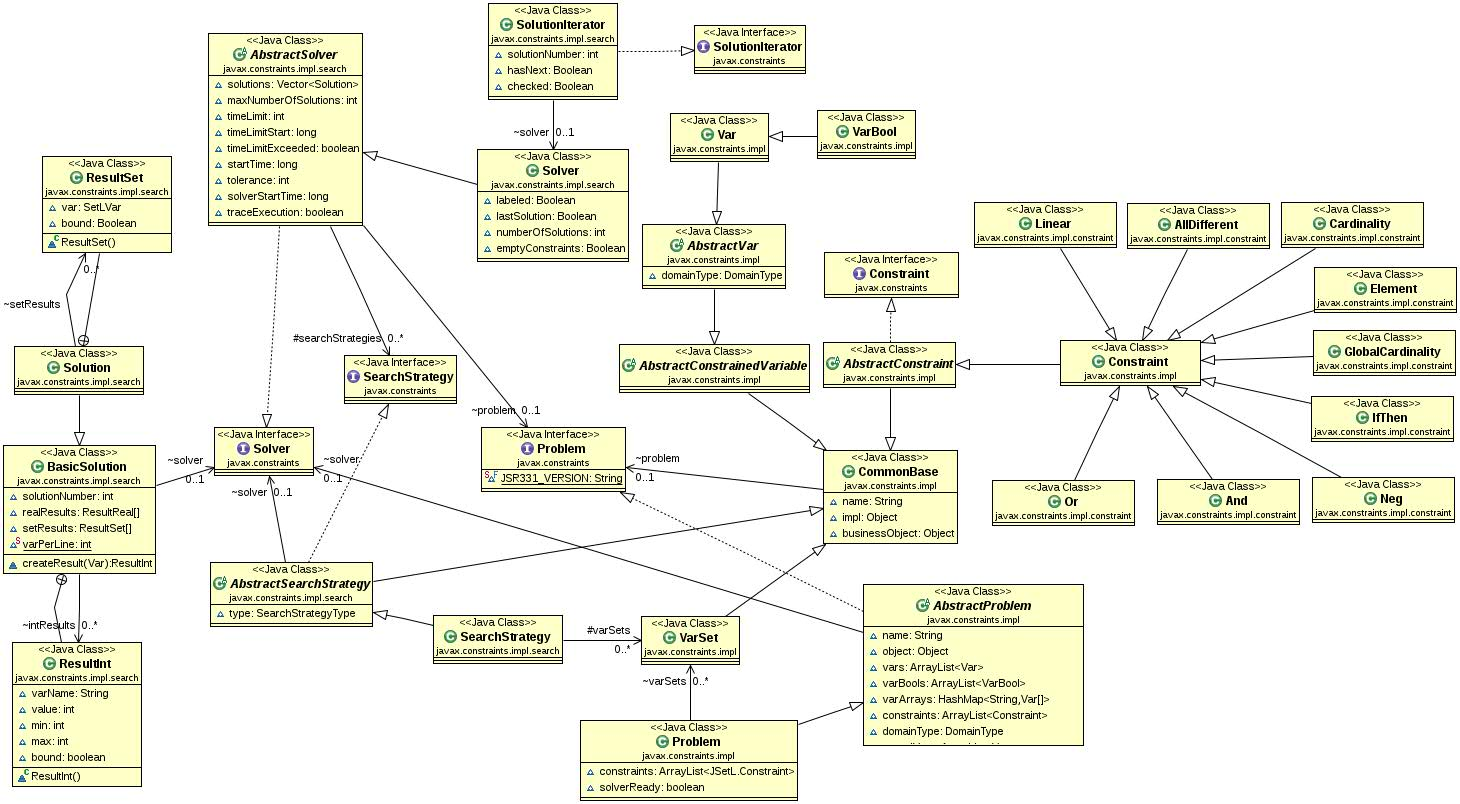
\includegraphics[scale=0.22]{../relazione/img/Progetto.JPG}
\end{center}
\end{frame}

\begin{frame}
\frametitle{Implementazione}
\framesubtitle{Class Diagram: definizione del problema}
\begin{center}
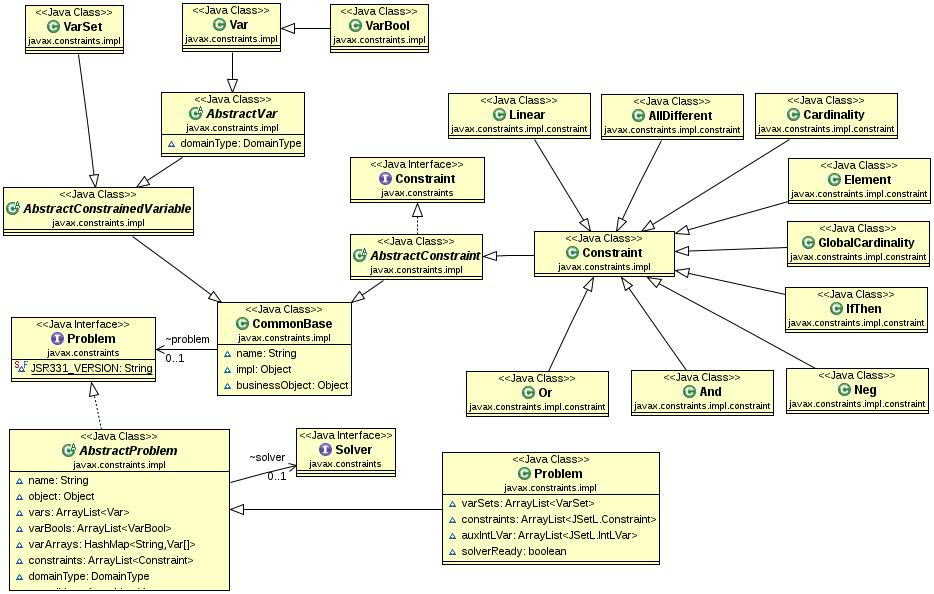
\includegraphics[scale=0.32]{../relazione/img/Problema.JPG}
\end{center}
\end{frame}

\begin{frame}
\frametitle{Implementazione}
\framesubtitle{Class Diagram: soluzione del problema}
\begin{center}
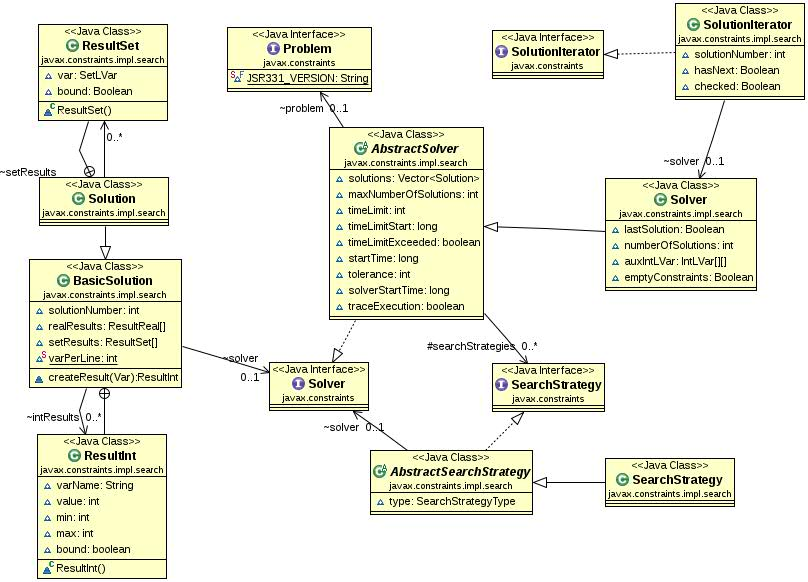
\includegraphics[scale=0.32]{../relazione/img/Soluzione.JPG}
\end{center}
\end{frame}

\begin{frame}
\frametitle{Implementazione}
\framesubtitle{Codifica}
Nella fase di codifica si sono implementate $18$ classi suddivise tra i
tre package richiesti:
\pause
\begin{block}{Definizione del problema}
\texttt{Problem}, \texttt{Constraint}, \texttt{Var}, \texttt{VarBool} e
\texttt{VarSet}.
\end{block}
\pause
\begin{block}{Vincoli}
\texttt{AllDifferent}, \texttt{Cardinality}, \texttt{Element},
\texttt{GlobalCardinality}, \texttt{Linear}, \texttt{And},
 \texttt{IfThen}, \texttt{Neg} e \texttt{Or}.
\end{block}
\pause
\begin{block}{Risoluzione}
\texttt{Solver}, \texttt{SearchStrategy}, \texttt{Solution} e
\texttt{SolutionIterator}.
\end{block}
\end{frame}


\begin{frame}[fragile]
\frametitle{Implementazione}
\framesubtitle{Mapping: disgiunzione}
\begin{columns}
\begin{column}{0.55\textwidth}
\begin{block}{Gerarchia}
Sia \texttt{Or} che \texttt{Constraint} estendono la classe astratta
fornita da JSR-331, che implementa l'interfaccia e si basa su
\texttt{CommonBase}.
\end{block}
\begin{block}{\texttt{CommonBase}}
\`E  una classe contenitore, utile alle implementazioni poiché
fornisce servizi \emph{getter} e \emph{setter}.
\end{block}
\end{column}
\begin{column}{0.4\textwidth}
\begin{flushleft}
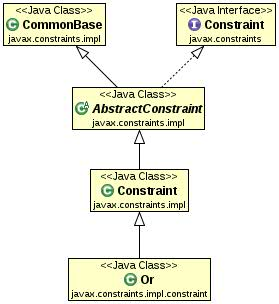
\includegraphics[scale=0.45]{../relazione/img/Or.JPG}
\end{flushleft}
\end{column}
\end{columns}
\end{frame}

\begin{frame}[fragile]
\frametitle{Implementazione}
\framesubtitle{Mapping: disgiunzione}
Dati due vincoli \texttt{c1} e \texttt{c2},  la classe \texttt{Or} mediante
il costruttore genera un nuovo vincolo \texttt{c} tale che:
\[\texttt{c} = \texttt{c1} \vee \texttt{c2}\]

\begin{lstlisting}[language = Java, linewidth = 200pt]
public Or(Constraint c1, Constraint c2) {
        super(c1.getProblem());
        Constraint result = (Constraint) c1.or(c2);
        setImpl(result.getImpl());
}
\end{lstlisting}

\pause
\begin{flushleft}
Il metodo \texttt{or(Constraint)} della classe \texttt{Constraint}.
\begin{lstlisting}[language = Java, linewidth = 280pt]
public Constraint or(javax.constraints.Constraint x) {
        JSetL.Constraint c1 = this.getConstraint();
        JSetL.Constraint c2 = ((Constraint) x).getConstraint();
        Constraint c = new Constraint(getProblem(), c1.or(c2));
        return c;
}
\end{lstlisting}
\end{flushleft}
\end{frame}




\begin{frame}[fragile]
\frametitle{Implementazione}
\framesubtitle{La classe \texttt{Solver}}
\begin{columns}
\begin{column}{0.55\textwidth}
\begin{block}{Gerarchia}
Estende \texttt{AbstractSolver} che non sfrutta la classe \texttt{CommonBase},
non è quindi prevista un'implementazione
specifica.
\begin{lstlisting}[language = Java, linewidth = 170pt]
public class Solver extends AbstractSolver {

  private SolverClass jsetlSolver;
  .
  .
\end{lstlisting}
Il solver JSetL è inserito tra gli attributi della classe.
\end{block}
\end{column}
\begin{column}{0.4\textwidth}
\begin{flushleft}
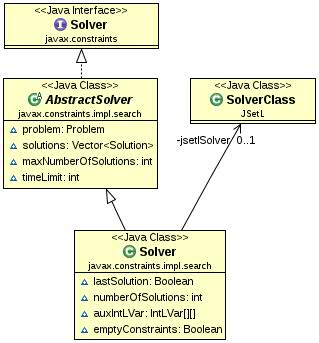
\includegraphics[scale=0.45]{../relazione/img/Solver1.JPG}
\end{flushleft}
\end{column}
\end{columns}
\end{frame}

\begin{frame}[fragile]
\frametitle{Implementazione}
\framesubtitle{La classe \texttt{Solver}}
\begin{columns}[t]
\begin{column}{0.5\textwidth}
\begin{block}{Costruttore}
Il costruttore della classe  istanzia il solver JSetL, quindi vi inserisce
tutti i vincoli salvati dal problema.
\end{block}
\end{column}
\begin{column}{0.4\textwidth}
\begin{lstlisting}[language = Java, linewidth = 130pt]
public Solver(Problem problem) {
  super(problem);
  jsetlSolver = new SolverClass();
  numberOfSolutions = 0;
  getProblemConstraints();
  setProblemConstraints();
  getAuxVariables();
}
\end{lstlisting}
\end{column}
\end{columns}

\pause

\begin{columns}
\begin{column}{0.5\textwidth}
\begin{block}{Ricerca di una soluzione}
Il cuore del metodo \alert{\texttt{findSolution}}, invoca la \texttt{solve}
di JSetL e quindi crea la soluzione con il relativo costruttore.
\end{block}
\end{column}

\begin{column}{0.4\textwidth}
\begin{lstlisting}[language = Java, linewidth = 140pt]
public Solution findSolution(ProblemState restoreOrNot) {
  .
  .
  jsetlSolver.solve();
  solution = new Solution(this,
               numberOfSolutions++);
  .
  .
\end{lstlisting}
\end{column}
\end{columns}
\end{frame}

\section{Conclusioni e lavori futuri}

\begin{frame}
\frametitle{Valutazione delle prestazioni}
\framesubtitle{Test semplici}
\begin{block}{Test semplici}
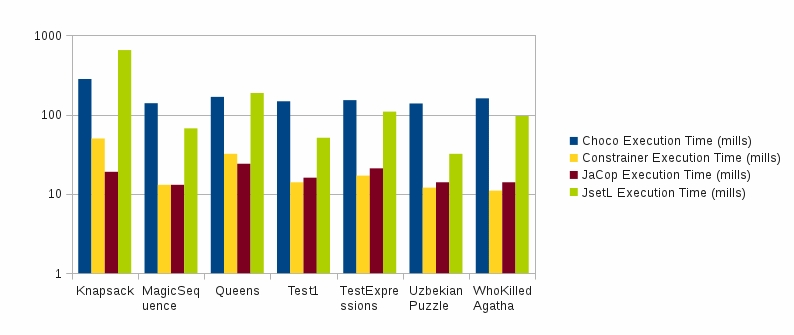
\includegraphics[scale=.4]{../relazione/img/grafico11.jpg}
\end{block}
\end{frame}

\begin{frame}
\frametitle{Valutazione delle prestazioni}
\framesubtitle{Test complessi}
\begin{block}{Test complessi}
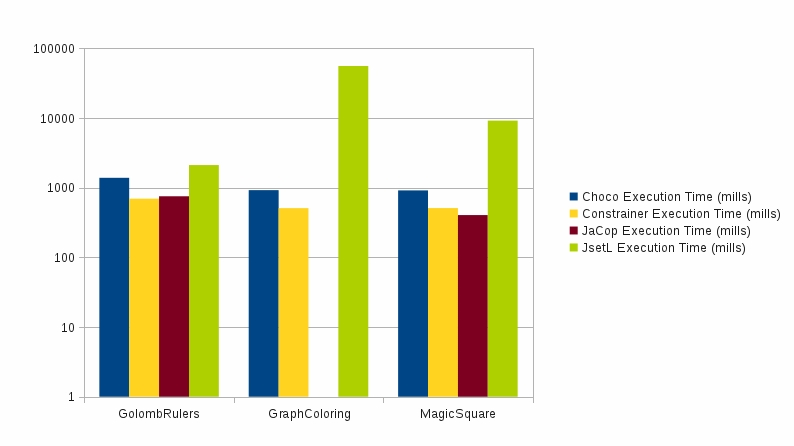
\includegraphics[scale=.35]{../relazione/img/grafico13.jpg}
\end{block}
\end{frame}

\begin{frame}
\frametitle{Conclusioni}
Il lavoro di tesi verte sui seguenti punti fondamentali:
\pause
\begin{itemize}%[<+->]
\item Studio della specifica JSR-331.
\item Studio del solver JSetL.
\item Realizzazione dell'implementazione.
\item Test di validazione e coverage.
\item Valutazioni delle prestazioni.
\item Comparazione con altri solver.
\end{itemize}

\begin{flushleft}
JSR-331 ha fornito un ottimo banco di prova per JSetL, nonché l'opportunità
di migliorarne alcuni aspetti.
\end{flushleft}
\end{frame}

\begin{frame}
\frametitle{Lavori futuri}
Si evidenziano i seguenti possibili sviluppi futuri:
\pause
\begin{itemize}%[<+->]
\item Estendere l'implementazione con funzionalità specifiche di JSetL non
previste dal JSR-331.
\item Mantenere allineata l'implementazione con gli sviluppi futuri della
specifica.
\item Valutare implementazioni alternative per la specifica.
\item Integrare nuove funzionalità offerte da JSetL.
\item Contribuire allo sviluppo del TCK.
\item Pubblicazione di un rapporto tecnico (in fase di stesura).
\end{itemize}
\pause
\begin{flushright}
\rm \LARGE \textit{Grazie!}
\end{flushright}
\end{frame}




\section{Appendice}

\begin{frame}[fragile]
\frametitle{Esempi}
\framesubtitle{Un esempio di CSP}
\begin{lstlisting}
    Problem p = new Problem("TestXYZ");
    Var x = p.variable("X", 0, 10);
    Var y = p.variable("Y", 0, 10);
    Var z = p.variable("Z", 0, 10);
    p.post(x,"<",y); 		// X < Y
    p.post(x.plus(y),"=",z); 	// X + Y = Z
    p.post(y,">",5);
    Var cost = p.variable("Cost", 2, 25);
    // Cost = 3XY - 4Z
    p.post(cost,"=",x.multiply(3).multiply(y).minus(z.multiply(4)));
    return p;

    Problem problem = defineCsp();
    problem.log("=== Optimal Solution:");
    Solver solver = problem.getSolver();
    Var costVar = problem.getVar("Cost");
    Solution solution = solver.findOptimalSolution(Objective.MAXIMIZE, costVar);
    if (solution == null)
            problem.log("No Solutions");
    else
            solution.log();
    problem.log("Cost=" + solution.getValue("Cost"));
    assertTrue(solution.getValue("Cost") == 23);
\end{lstlisting}
\end{frame}

\end{document}
